% !TEX program = pdflatex
% !BIB program = bibtex
% !TEX encoding = UTF-8 Unicode
% !TEX spellcheck = en_us

\documentclass[10pt, twocolumn, journal]{IEEEtran}
\usepackage[utf8]{inputenc}
\usepackage[T1]{fontenc}
\usepackage{cite}
\usepackage{graphicx}
\usepackage{caption}
\captionsetup{font=footnotesize, justification=justified}
\usepackage{enumitem}
\usepackage{amsmath}

% Myriad Pro Font
\usepackage{MyriadPro}
%or
%\usepackage{mdsymbol}

\title{Flexible API for IoT Services with Named Data Networking}
\author{
    \IEEEauthorblockN{Christopher Horn}\\
    \IEEEauthorblockA{
        University of Lübeck, Germany\\
        christopher.horn@student.uni-luebeck.de
    }
}

\begin{document}
\maketitle
\thispagestyle{empty}
\begin{abstract}
The Internet of Things (IoT) is changing our lives by offering different devices that can sense the environment and monitor network events. These devices are usually wirelessly connected to the internet. The IoT devices have applications and services that provide users with collected data and information. This paper shows the development of an Application Programming Interface (API) for services using Named Data Networking (NDN). NDN allows for smart transmission of data by utilizing content names. Additionally, a new layer is introduced in the IoT-NDN architecture to enhance communication between devices and services in the IoT ecosystem. 
\end{abstract}

\section{Introduction}
The development of Internet of Things (IoT) architecture and design is benefitting our activities through IoT applications and services. IoT devices, when connected to the internet, gather data to monitor different environmental events. However, there are ways to facilitate the integration of devices and IoT applications using internet-based methods. A crucial aspect is defining the interfaces for applications and services that operate on devices. The Named Data Network (NDN) which is a version of the Information Center Network (ICN) \cite{ahlgren2012survey} represents a solution to address these challenges \cite{zhang2010named} while also being adaptable to future network advancements. Following this progress, in IoT essential concepts of the NDN system have been implemented, such as naming and forwarding.

\section{IoT with Named Data Networking (NDN)}
The Internet was initially created for tasks such as computer messaging. However, it has evolved to handle data exchanges like multimedia files and big data. This evolution necessitated a redesign, which led to the development of NDN. NDN is a network architecture that focuses on communication-based data names of the traditional host-to-host model used by TCP/IP. In NDN, structured names are used in Interest and Data Packets, which are managed through three tables; Content Store (CS) caches all in-coming data, Pending Interest Table (PIT) keeps track of the forwarding including the faces ID which the Interest coming from, and Forwarding Information Base (FIB) is as a routing table, it routes and forwards the content based on content names. Responses are based on the availability of the requested data in CS or PIT. Intermediate nodes also cache data to reduce repeated access.

In the context of IoT-NDN systems, NDN offers communication features for devices that have limited resources \cite{hail2015iot}. By addressing the requirement of efficient data caching and transmission in IoT, this approach proves advantageous for energy-constrained devices. It improves access to content while reducing network congestion. The lightweight design of IoT-NDN is well-suited for networks with hops in various scenarios of IoT applications.

\section{API for IoT Services}
This section introduces an API that can be used to integrate services and protocols. IoT services are essential for internet-based systems in the future, as they perform tasks and provide precise information. Examples of these services include network time synchronization and location detection services. Although there is a debate about their definition, they essentially act as individual devices that offer access to their resources for delivering information. These IoT services provide data from device sensors and network environments, which can assist in decision-making processes, such as in healthcare.

The proposed API is designed to be adaptable for any service within the IoT-NDN system, making it easier to share and retrieve information from integrated services. Figure 1 illustrates the role of this API in IoT-NDN for providing services. Its cost-effectiveness and flexibility make it advantageous across sectors like cities and homes. The API's flexible interfaces between layers enhance the reliability and efficiency of systems.

\begin{figure}[ht]
    \centering
    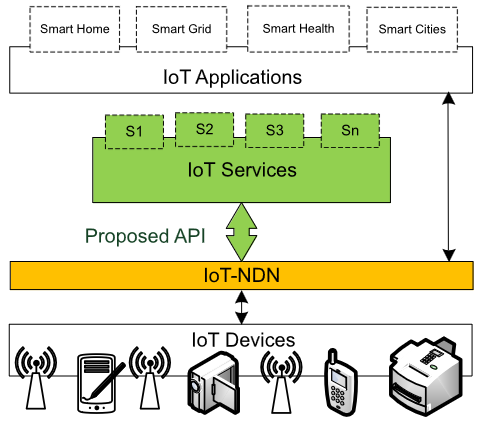
\includegraphics[width=0.4\textwidth]{figure_1.png}
    \caption{The proposed API for IoT-Services using IoT-NDN}
    \label{fig:figure_1}
  \end{figure}

This paper wants to emphasize the significance of service-oriented integration in the field of IoT, where services play a crucial role and can be programmed as smaller system modules. Despite the limitations of devices and due to resource constraints, the suggested services layer efficiently combines services. For instance, it enables real-time protocols and smart technology movement with the potential for expansion into tasks. The incorporation of services into devices does pose challenges. However, IoT-NDN on each device tackles this issue by accommodating applications and services. Once registered through the API these services can effortlessly receive data updates, such as network time synchronization. Moreover, the API is flexible enough to support higher-level device protocols that facilitate communication between applications and hardware.

\section{Implementation}
\subsection{Naming Concept for IoT-Services}
NDN offers more flexible data requests than traditional internet structures, using hierarchically structured, human-friendly names that are location-independent. This structure allows better control over data transmission between devices. NDN supports saving and retrieving data copies across devices, reducing network traffic. Names in IoT systems typically represent specific tasks or events. For example, an Interest name in the IoT-NDN system might request network time sensor information, as illustrated in Figure 2. The naming structure comprises several components, facilitating easy understanding and response to data requests \cite{amadeo2014named}.

\begin{figure}[ht]
    \centering
    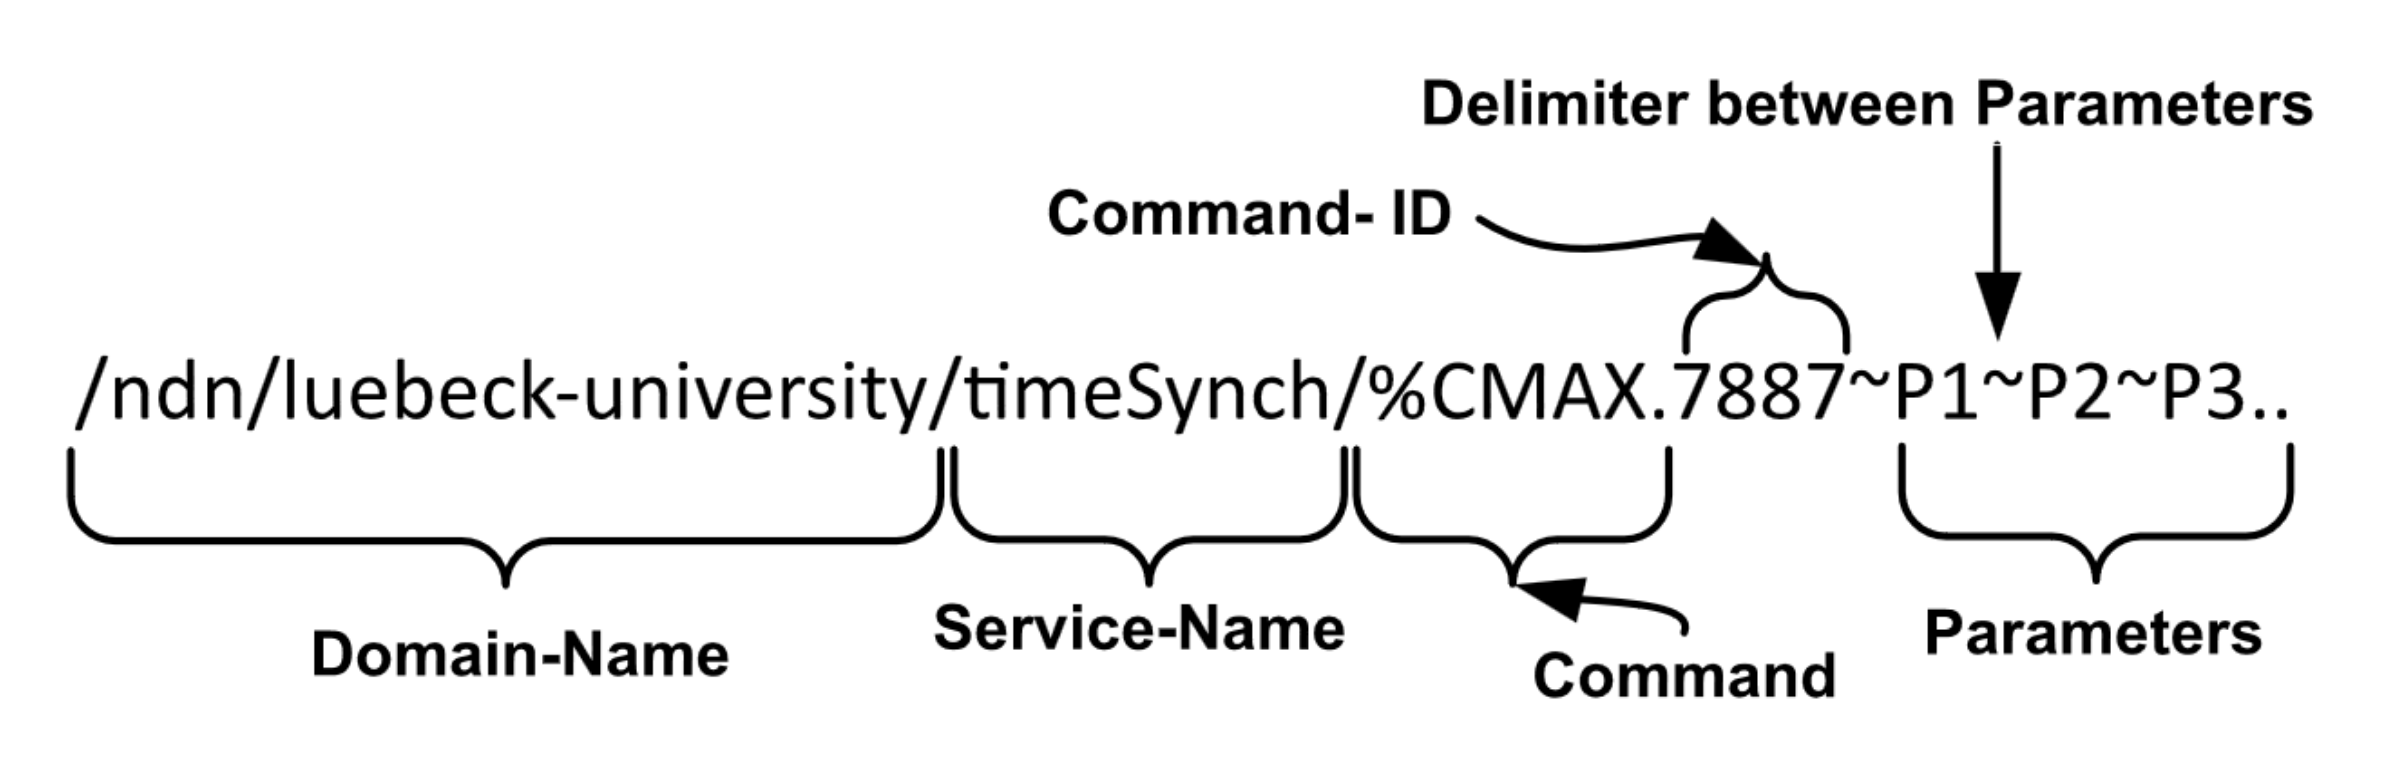
\includegraphics[width=0.4\textwidth]{figure_2.png}
    \caption{Name Structure for IoT services including commands and their parameters}
    \label{fig:figure_2}
  \end{figure}

The name includes a Command Concept with three parts: 
\begin{enumerate}[label=\arabic*.), leftmargin=1cm]
    \item COMMAND: A six-letter code for specific tasks, encoded in Type-Length-Value (TLV) format \cite{zhang2010named}.
    \item COMMAND ID: Identifies the message or command sent from the service.
    \item COMMAND PARAMETERS: Helps in processing the command on the sink device or intermediate nodes.
\end{enumerate}

This structure can be extended to transmit various information types, allowing users to access general service information.

\subsection{Deployment of IoT Services}
IoT services considered small software units, monitor events and provide specific knowledge thereby enhancing decision-making efficiency in IoT systems. The API's architecture and functions for registering new services are shown in Figure 3. For example, it demonstrates the exchange of Interest/Data packets between IoT-Services and IoT-NDN layers. Services are registered using the naming structure from section IV-A, and the IoT-NDN system searches for matching Data in the CS or forwards Interests based on NDN principles.

\begin{figure}[ht]
    \centering
    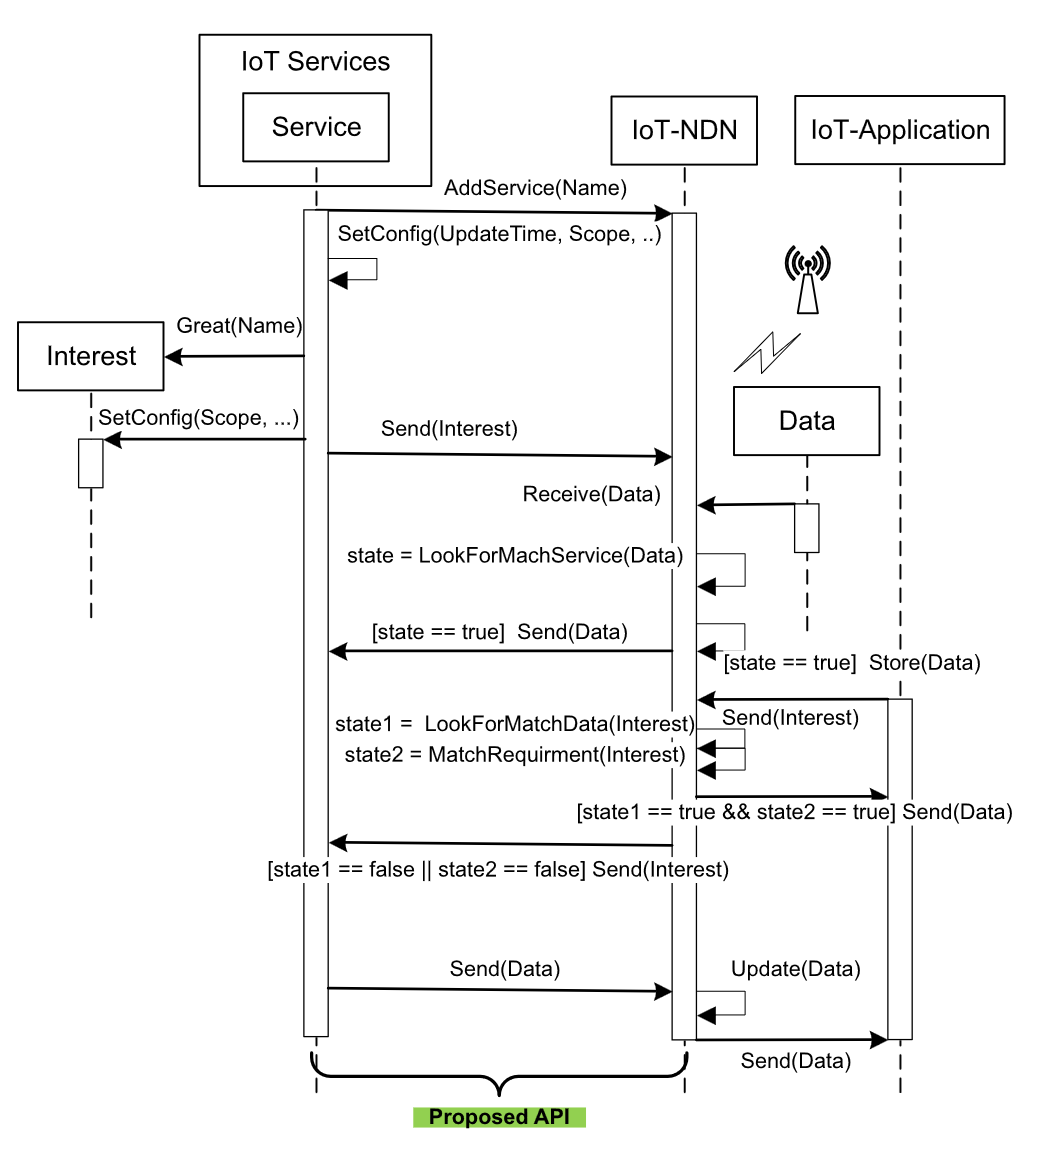
\includegraphics[width=0.4\textwidth]{figure_3.png}
    \caption{Example of Service Integration and Exchange of Interest and
    Data Packets in IoT-NDN with the proposed API}
    \label{fig:figure_3}
  \end{figure}

\raggedright
\setlength{\parindent}{1em}
Example of Service Registration: In this example, a network time synchronization on Internet-connected devices is considered. The service name is defined as \{\textmd{/ndn/luebeck-university/NetworkTimeSynch/\%SCONFI.1$^{\sim}$5s}\}, including a setConfig command with a 5-second update interval. After integrating the service, the IoT-NDN system sends Interests to neighboring nodes based on this configuration. 

\section{Conclusion}
This work introduces an Application Programming Interface (API) for IoT services utilizing Named Data Networking (NDN), offering a simple and flexible integration of diverse services for heterogeneous IoT devices. The NDN approach is highlighted as efficient and intelligent, with the IoT-NDN system's benefits briefly summarized. The NDN naming concept has been enhanced with an additional command system for effective service control via the API. A network time synchronization service example demonstrates the API's flexibility and integration benefits. Plans include testing the API with more services and further developing the implementation to enhance ease of use.
% Literaturverzeichnis
\bibliographystyle{IEEEtran}
\bibliography{references} % Verweisen Sie auf Ihre BibTeX-Datei

\end{document}
